\documentclass{article}
\usepackage[utf8]{inputenc}
\usepackage{polski}
\usepackage{graphicx}
\usepackage{listings} 

\title{Sprawozdanie FTP}
\author{Jan Bronicki 249011\\Poniedziałek, 15:15 - 16:55 TN}
\date{}


\begin{document}

\maketitle

\section{Wstęp}
FTP (File Transfer Protocol) to protokół, który umożliwia połączenie z serwerem komputerowym w celu przesłania plików. W internecie istnieje wiele darmowych aplikacji, tzw. klientów FTP (np. WinSCP) służących do zarządzania plikami na serwerze. Ich konfiguracja sprowadza się do instalacji i ustanowienia połączenia z serwerem.
\section{Serwer FTP}


Na początku upewniamy się, że nasz system jest zupdateowany:

\begin{lstlisting}
    $ sudo apt-get update
\end{lstlisting}

\begin{lstlisting}
    $ sudo apt-get upgrade
\end{lstlisting}

Teraz, instalujemy jeden z programów umożliwiających naszemu Ubuntu zostanie serwerem FTP. Zainstalujemy vsftd
\begin{lstlisting}
    $ sudo apt-get install vsftpd
\end{lstlisting}
Następnie po instalacji sprawdzamy status działania usługi za pomocą komendy:
\begin{lstlisting}
    $ sudo systemctl status vsftpd
\end{lstlisting}
Jeśli wszystko poszło sprawnie taki powinniśmy dostać output. Oznacz to, że server działa:

\begin{figure}[h!]
    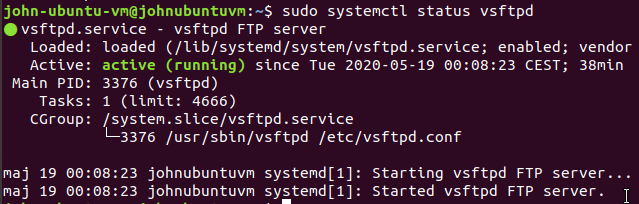
\includegraphics[scale=0.6]{ssytemctl.png}
    \centering
\end{figure}
 \newpage
Następnie, aby połączyć się z serverem i wymieniać z nim informacje będziemy potrzebować programu, który (najlepiej w sposób łatwy, czyli graficzny) nam to umożliwi. W moim przypadku będzie to darmowa, open-source Filezilla.

\begin{figure}
    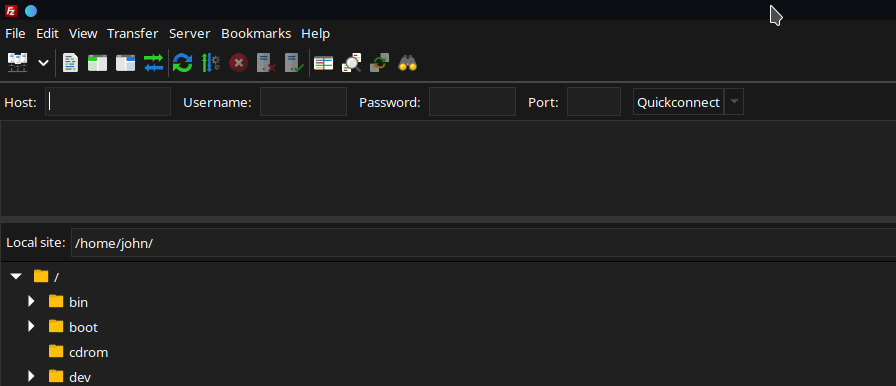
\includegraphics[scale=0.5]{zilla.png}
    \centering
\end{figure}

Aby połączyć się z naszym serwerem będziemy potrzebować jego adresu. Do tego możemy użyć np. komendy:
\begin{lstlisting}
    $ ifonfig
\end{lstlisting}
Dla mnie, server, które znajduje się na maszynie wirtualnej ubuntu (na tej samej sieci) ma adres:
\begin{lstlisting}
    192.168.1.8
\end{lstlisting}
Połączenie FTP zachodzi po 21 porcie.
Udało nam się pomyślnie połączyć z uzytkownikiem bob na serverze. Zostajemy przeniesieni do jego katalogu domowego:
\begin{figure}[h!]
    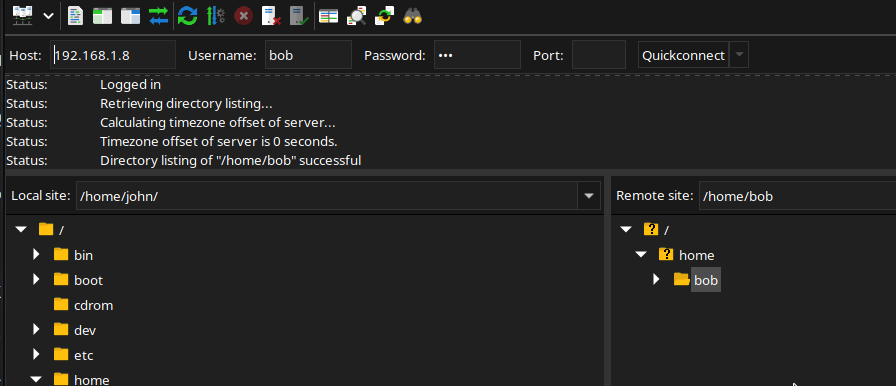
\includegraphics[scale=0.5]{bobzilla.png}
    \centering
\end{figure}
\newpage

Ale bez modyfikacji konfiguracje jedynie co jesteśmy w stanie robić to pobierać pliki z servera (w tym przypadku katalogu domowego bob'a). Dlatego, aby móc edytować, dodawać itp pliki udajemy się do pliku konfiguracyjnego. Otwieramy go używając nano:
\begin{lstlisting}
    $ sudo nano /etc/vsftpd.conf
\end{lstlisting}

Następnie odkomentowujemy linię broniącą nas przed edycją plików:
\begin{figure}[h!]
    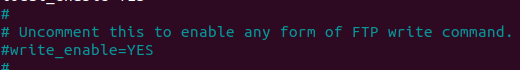
\includegraphics[scale=1]{uncom.png}
    \centering
\end{figure}
\begin{figure}[h!]
    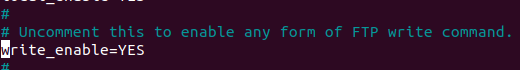
\includegraphics[scale=1]{nomlin.png}
    \centering
\end{figure}
Następnie musimy zresetować servera, aby nowa konfiguracja weszła w życie.
\begin{lstlisting}
    $ sudo systemctl restart vsftpd 
\end{lstlisting}
Po tym możemy modyfikować pliki boba.
Po skończeniu pracy wyłączamy serwer:
\begin{lstlisting}
    $ sudo systemctl stop vsftpd 
\end{lstlisting}
\end{document}